\documentclass[letterpaper]{article}
\usepackage[utf8]{inputenc}
\usepackage[parfill]{parskip}    % Activate to begin paragraphs with an empty line rather than an indent
\usepackage{graphicx}
\usepackage{amssymb}
\usepackage{amsmath}
\usepackage{amsthm}

\usepackage{afterpage}

\usepackage{algorithm}
\usepackage{algpseudocode}

\usepackage{verse}

\newtheorem{theorem}{Theorem}[section]
\newtheorem{corollary}{Corollary}[theorem]
\newtheorem{lemma}[theorem]{Lemma}

\theoremstyle{remark}
\newtheorem*{remark}{Remark}

\usepackage{epstopdf}
\usepackage{circuitikz}
\usepackage[separate-uncertainty = true,multi-part-units=single]{siunitx}
\usepackage{booktabs}
\usepackage{enumitem}
\usepackage[toc,page]{appendix}
\usepackage{color}
\usepackage{pgfplots}
\usepackage{pgfplotstable}
\usepackage{caption}
\usepackage{subcaption}
\usepackage{url}
\usepackage{multirow}
\usepackage{makecell}
\usepackage[round]{natbib}   % omit 'round' option if you prefer square brackets
\usepackage{titling}
\usepackage{siunitx}

\usepackage{setspace}
% \doublespacing
\usepackage{float}

\pgfplotsset{compat=1.14}


\usepackage{fancyhdr}

\pgfplotscreateplotcyclelist{grayscale}{
    thick,white!10!black,mark=x,mark options=solid, dashed\\%
    thick,white!20!black,mark=o,mark options=solid\\%
}


\newcommand{\answer}[1]{\framebox{$\displaystyle #1 $}}

 
\pagestyle{fancy}
\fancyhf{}
\rhead{David Shi}
\lhead{CS61C}
\cfoot{\thepage}

\title{Lecture 4 - Notes}
\author{David Shi}
\date{June 2019}
\begin{document}

\maketitle

\section{Overview}
In the last lecture, we mainly focused on Pointers and implementations of pointers such as arrays and strings. We also discussed many of the reasons that pointers are a significant pitfall for errors in C programming. In this lecture, we will focus more on memory allocation and behavior as we wrap up our last lecture focused on C.

\section{C Memory Layout}
\begin{center}
    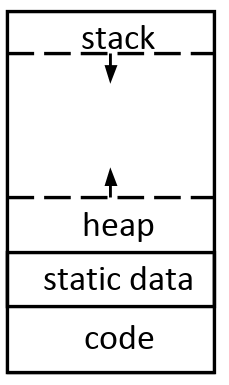
\includegraphics[scale=.5]{memorylayout}
\end{center}
The above figure summarizes the address space of a program. Here is a summary of the 4 regions of address space:
\begin{itemize}
    \item \textbf{Stack:} Local Variables, grows downward
    \item \textbf{Heap:} Space requested with malloc() and used with pointers, spaced dynamically, grows upward
    \item \textbf{Static Data:} Global and static variables. Never changes in size
    \item \textbf{Code:} loaded when program starts, does not change
\end{itemize}

Variables that are declared outside of a function are placed in the static data

Variables that are declared inside of functions are placed in the stack. When the function returns, the variables are freed

Variables that are dynamically allocated are placed in the heap. We will cover what this means shortly

\subsection{Stack}
Each stack frame is a contiguous block of memory holding all of the local variables of a single procedure.

\begin{center}
    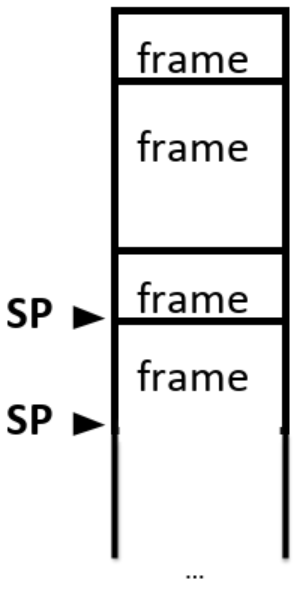
\includegraphics[scale=.5]{stack}
\end{center}

A stack frame includes the location of the caller function, function arguments, and space for local variables. It is similar to the environment frames we learned about in CS61A.

A stack pointer points to the lowest current stack frame is. When the procedure ends, the stack pointer moves back (pointing to garbage), to free up memory for future frames. The stack uses a LIFO (Last in first out) data structure, where the last function called in a single procedure gets returned last. We learned about this concept in CS61A as well.

\textbf{WARNING:} Never return a pointer to a local variable in a function. Since once the function returns, the local variable that the poitner points to gets wiped and will be garbage.

\subsection{Static Data}
The Static Data is a place for variables that persist across separate procedures. These data are not subject to disappearing due to function calls. Examples include string literals and global variables. The sizes cannot change, but sometimes the data can change.

\subsection{Code}
The code is a place for a copy of our code. This copy is stored as data, and does not change while running.

\subsection{Addresses and Endianness}
The size of an address depends on the computer's architecture. If a machine is \textbf{byte-addressed}, then each address points to a unique byte. 

Endianness refers to the storage in memory for values that occupy multiple bytes. The two types of Endianness are \textbf{Big Endianness} and \textbf{Little Endianness}. The two types refer to how numerical significance is associated with memory addresses.

Big Endianness assigns descending numerical significance with ascending memory addresses. An inverse relationship

Little Endianness assigns ascending numerical significance with ascending memory addresses, a linear relationship.

\section{Dynamic Memory Allocation}
Dynamic memory allocation is for when we want persisting memory (like static data) when we don't know the size at compile time. Examples include user input or input files. This wouldn't work in stack because the stack doesn't persist. Dynamically allocated memory goes into the Heap in our memory space, which is more permanent than the stack. Our heap should take up as much memory as possible without interfering with the stack, and it grows upward towards the stack.

Since integer sizes are machine dependent, we need to use the sizeOf() operator.

\section{Allocating Memory}
Our 3 functions for dynamically allocating memory include malloc(), calloc(), and realloc(), as well as free for freeing data.

\subsection{malloc(n)}
This function allocates a continuous block of n bytes of uninitialized data to our memory. This memory will contain garbage as it is uninitialized. This function call returns pointer that points to the beginning of the allocated block, sort of like how we have been picturing memory as an array. If the request to allocate memory fails, the pointer will point to NULL. We should check for this potential bug.

malloc(n) is almost always used for arrays or structs. It is good practice to use sizeOf() and type casting when calling malloc for the value of n.

\subsection{free(p)}
We release memory from our heap using the free(p) operator. We can pass in pointer p to the beginning of the allocated block to release the entire block. p must point to the beginning of the originally called block for free to work. Otherwise, an exception gets thrown. Releasing memory is good practice as memory on a computer is limited and we want as much memory available as possible at all times.

We should not use free on a block that has already been released or on a pointer that is NULL. Also, incrementing our original pointer p is a bad idea. We should use a separate pointer in order to later release the block p.

\subsection{calloc(size_t nmemb, size_t size)}
Similar to malloc, except it initializes all memory to 0 rather than not initializing at all. nmemb refers to the number of members, while size refers to the size of each member. It returns a block of data of all 0s for nmemb members of size size.

\subsection{realloc(void *ptr, size_t size}
This function is useful when we need more or less memory in an array. It takes in a pointer that was returned by malloc, calloc or realloc and a new size, and returns a new pointer with size space and copies any contents from ptr.

\section{Memory Problems}
The most common memory error we will encounter in this class is the Segmentation Error, which was previously mentioned. A seg error is an error when a program tries to access memory not allocated to it.

Common reasons for memory bugs include the following:
\begin{itemize}
    \item Using uninitialized values (values that are garbage or point to garbage)
    \item Using unallocated memory (segmentation error)
    \item Freeing invalid memory (either already freed or null)
    \item Memory leaks (losing our original pointer, making the block impossible to free)
\end{itemize}

\section{Linked Lists}
We studied an implementation of Linked Lists in C that utilizes structs, pointers, and memory allocation. I would recommend reading the slides themselves (slides 50-54) as this was more of a demo than content. 

Link to slides: https://drive.google.com/file/d/1i\_4RwXOTWsOZUFWpl24fwd4alY2QIzEG/edit
\end{document}